% =====================================================================
%  CHAPTER 7 - RESULTS AND DISCUSSION
% =====================================================================
\clearpage
\chapter{Results and Discussion}

This chapter reports the measurements made on the cloud test bed of
Section~6.4 and the offline evaluation of semantic deduplication. Unless
stated otherwise, the configuration is three engine replicas, 16 shards and
four workflow and eight activity workers per shard (written r3/S16/w4x8),
and the workload is the delivery workflow of Section~5.8. Values are means of
three trials, with the range given where it is informative. All results
describe this configuration on this hardware; Section~\ref{sec:validity}
discusses how far they generalise.

\section{Latency Floor}

With one workflow in flight at a time, the median end-to-end latency was
2.21\,s (p99 4.3--4.4\,s), while the engine and database hosts were below
5\% CPU. Offering 1 workflow per second in open loop raised the median by
only 4--9\%. The floor is therefore not set by any resource.
Fig.~\ref{fig:floor} decomposes it using the timestamps in the event journal.
Each activity takes about 200\,ms from being scheduled to being recorded as
complete, most of which is the simulated service time and the activity
worker's poll interval. A fenced decision commit takes 33--38\,ms. The largest
single component is the lag of the 50\,ms preparation timer, which fired a
median of 580\,ms late; the due-timer scanner runs once per second, so a timer
waits on average half a second for the next scan.

\begin{figure}[htbp]
  \centering
  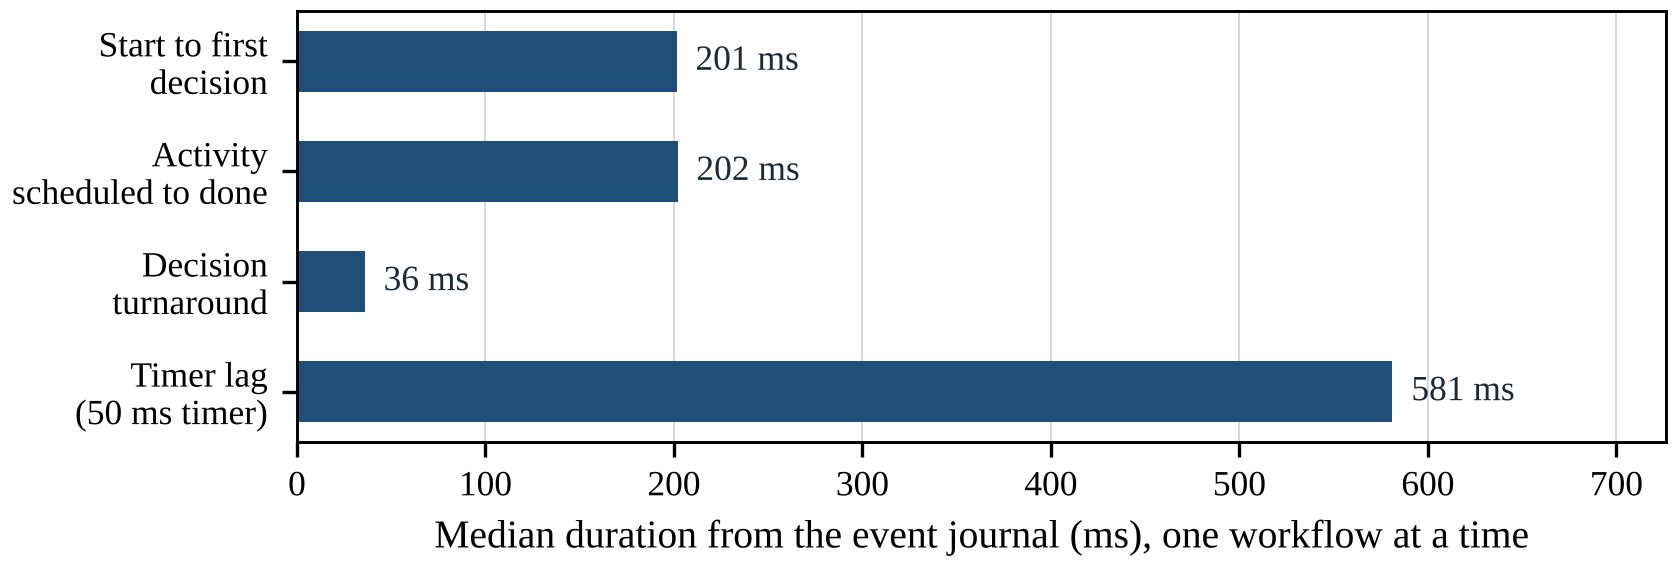
\includegraphics[width=0.9\linewidth]{figures/fig_7_8_latency_floor.png}
  \caption[Components of the latency floor]{Components of the latency floor
    at one workflow in flight (Stage~C).}
  \label{fig:floor}
\end{figure}

The floor is therefore a consequence of polling, and could be lowered by
notifying workers of new tasks and timers instead of having them poll, for
example with PostgreSQL's \cd{LISTEN}/\cd{NOTIFY}. Section~\ref{sec:closed}
shows the same effect from the other side: under moderate load the median
latency falls below the floor, because busy workers find work on their first
poll and do not back off.

\section{Idle Overhead}

Because workers poll, an idle cluster is not silent. Fig.~\ref{fig:idle}
shows the transactions committed per second by the database with no workload
for five configurations. At the default configuration the idle rate was
251\,commits/s at about 1\% database CPU. The rate grows with the number of
workers (165, 251 and 443\,commits/s for 2+4, 4+8 and 8+16 workers per
shard) and, at a fixed total of 192 workers, with the number of shards (251,
304 and 410\,commits/s for 16, 32 and 64 shards), because each shard adds a
timer scanner and a lease renewal. The trials were very repeatable, within
2\,commits/s of each other.

\begin{figure}[htbp]
  \centering
  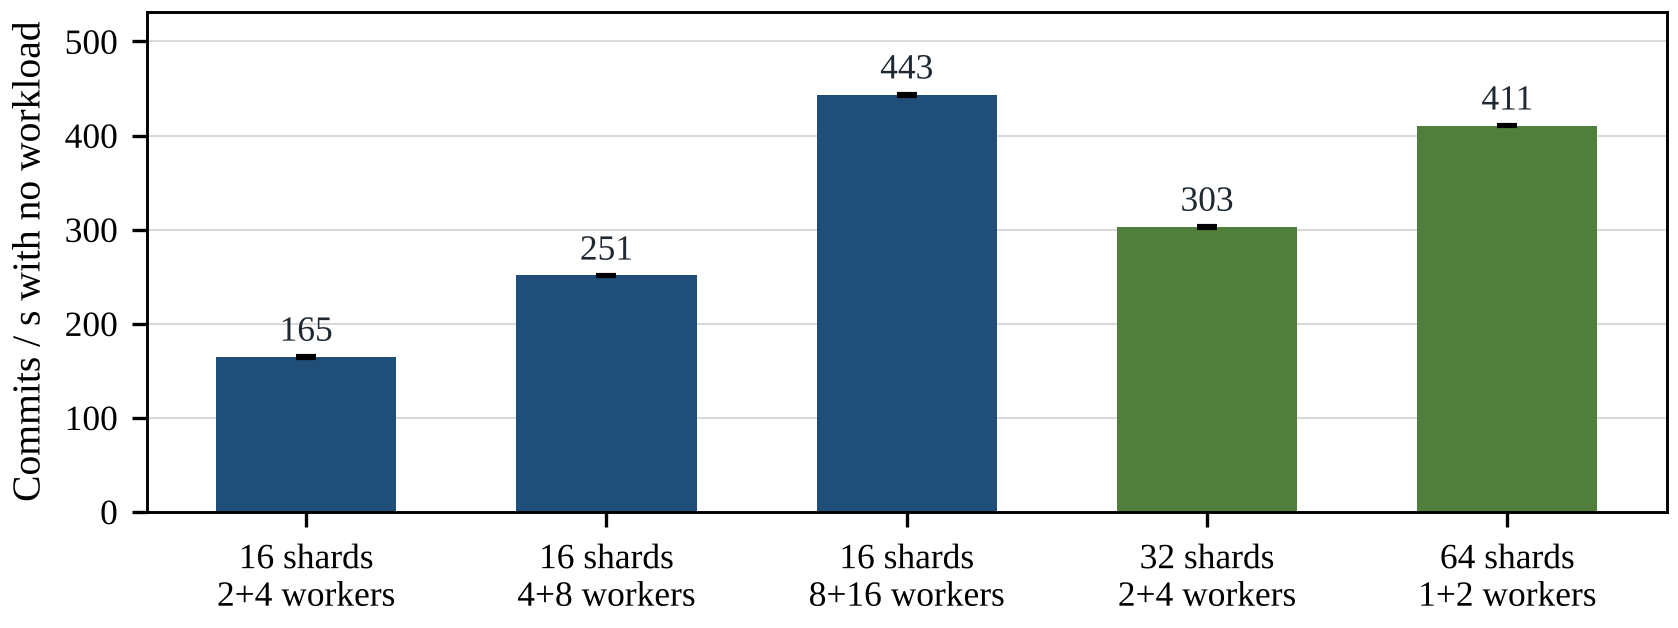
\includegraphics[width=0.85\linewidth]{figures/fig_7_5_idle_cost.png}
  \caption[Idle database load]{Database commits per second with no workload
    (Stage~B, three trials each).}
  \label{fig:idle}
\end{figure}

The cost is small in CPU but it is not small in transactions, and it is paid
on every host that runs the database whether or not any work is being done.
It is the price of using a table as a queue without a notification channel.

\section{Closed-Loop Capacity}
\label{sec:closed}

Fig.~\ref{fig:closed} and Table~\ref{tab:closed} give throughput and latency
as the number of concurrent workflows $c$ was increased. Up to $c=256$,
throughput grew almost linearly with $c$ and the median stayed near 2\,s,
which is what Little's law predicts for a system whose latency does not
change: $256 / 2.0\,\text{s} \approx 128$ workflows/s against the 131
measured. In this range the system is limited by latency, not capacity.

\begin{figure}[htbp]
  \centering
  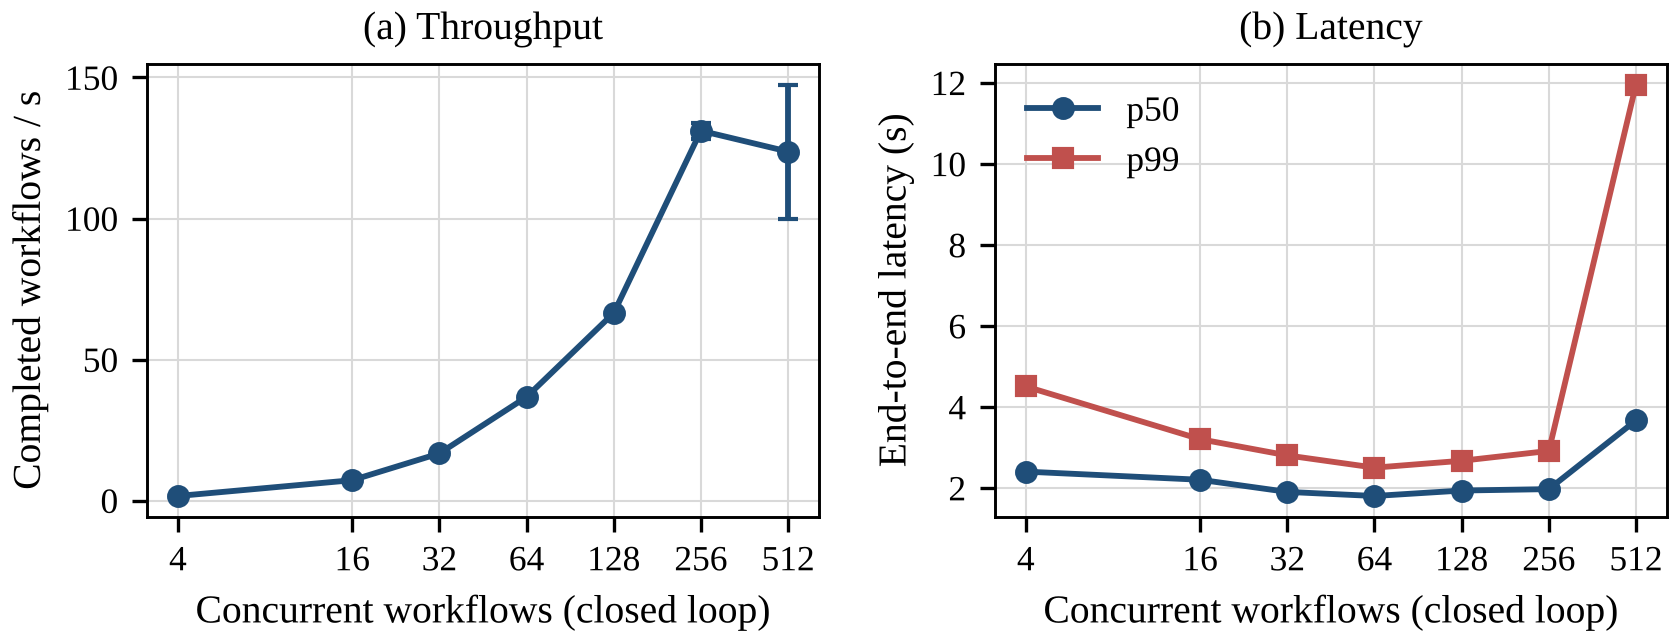
\includegraphics[width=0.9\linewidth]{figures/fig_7_1_closed_loop.png}
  \caption[Closed-loop throughput and latency]{Closed-loop throughput and
    latency against concurrency (Stage~D).}
  \label{fig:closed}
\end{figure}

\begin{table}[htbp]
  \centering
  \caption{Closed-loop results (r3/S16/w4x8)}
  \label{tab:closed}
  \small
  \begin{tabular}{@{}rrrrrr@{}}
    \toprule
    $c$ & \textbf{Workflows/s} & \textbf{p50 (s)} & \textbf{p99 (s)} &
      \textbf{DB CPU (\%)} & \textbf{Commits/s} \\
    \midrule
    4   & 1.6   & 2.41 & 4.51 & 4      & 481 \\
    16  & 7.2   & 2.21 & 3.21 & 8      & 1,209 \\
    64  & 36.8  & 1.80 & 2.50 & 22     & 4,100 \\
    128 & 66.5  & 1.9--2.0 & 2.6--2.7 & 41--52 & 7,150 \\
    256 & \textbf{131.1} & 1.9--2.0 & 2.7--3.1 & 74--96 & 13,200 \\
    512 & 123.7 & 3.1--4.1 & 8.8--14.0 & 96 & 18,400--20,100 \\
    \bottomrule
  \end{tabular}
\end{table}

At $c=512$ the mean throughput was lower than at 256 and varied widely
between trials (151, 107 and 113 workflows/s), while p99 rose by three to
five times. The first screening trial at 512 had suggested that throughput
was still rising; the repeated trials showed that it was not. This is why the
knee was taken from repeat means. The sustainable closed-loop capacity of
this configuration is therefore about 131 workflows/s at $c=256$.

Fig.~\ref{fig:resources} shows where the capacity goes. The database host
reached 84\% CPU on average at $c=256$ and 96\% at 512, while the busiest
engine node stayed below 63\% and the load generator below 30\%. The engines'
connection pools began to run empty at the same point, so the database and
the pools saturate together. The wait profile of the database
(Fig.~\ref{fig:waits}) changes in a consistent way: at low load almost all
sampled waits are for WAL flushes to disk, while from $c=128$ onwards waits
on the WAL write lock and on row locks dominate. The row-lock waits are
consistent with the fencing check, which serialises the commits of each
shard on its lease row, although the sampling did not identify the rows.

\begin{figure}[htbp]
  \centering
  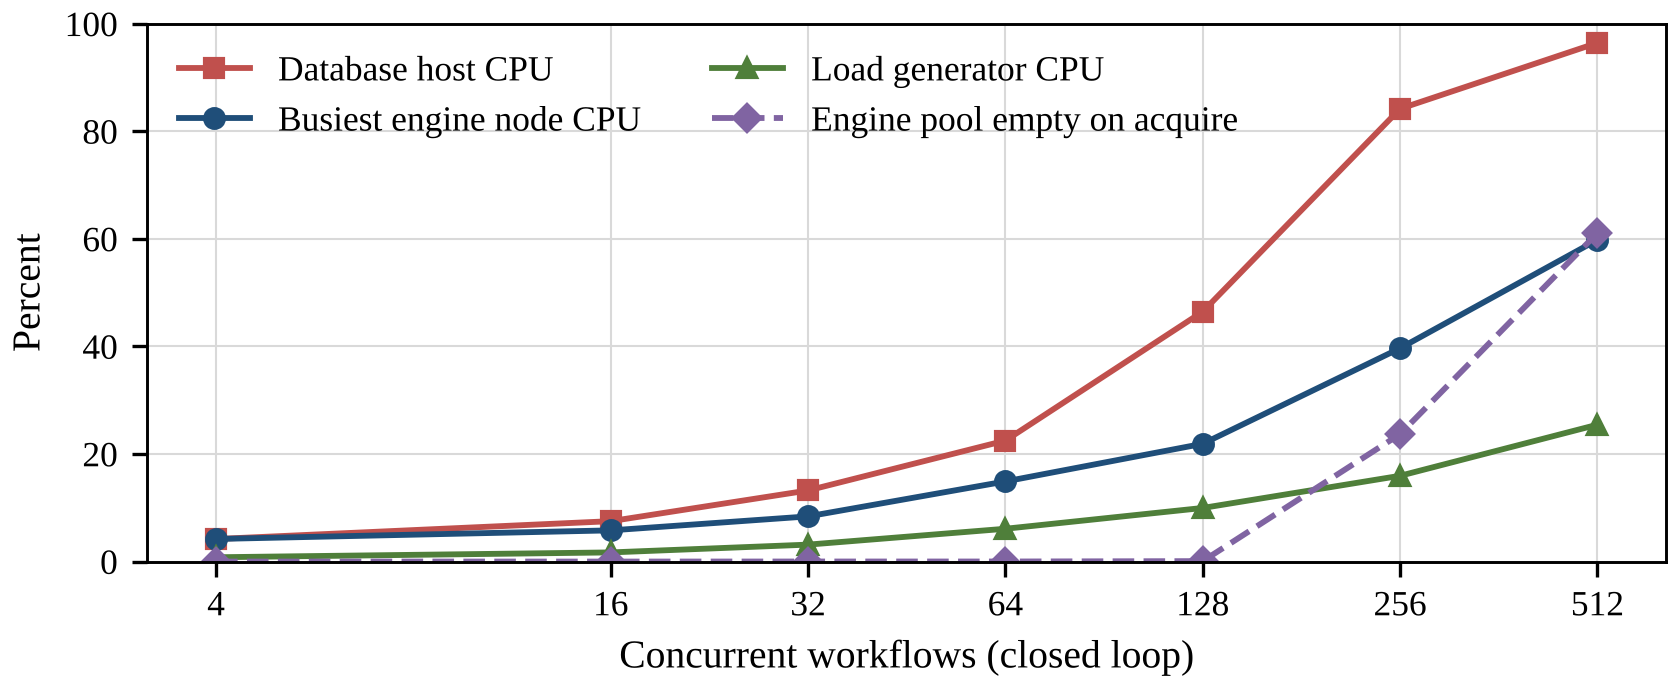
\includegraphics[width=0.9\linewidth]{figures/fig_7_2_resources.png}
  \caption[Resource use against concurrency]{Resource use against
    concurrency (Stage~D).}
  \label{fig:resources}
\end{figure}

\begin{figure}[htbp]
  \centering
  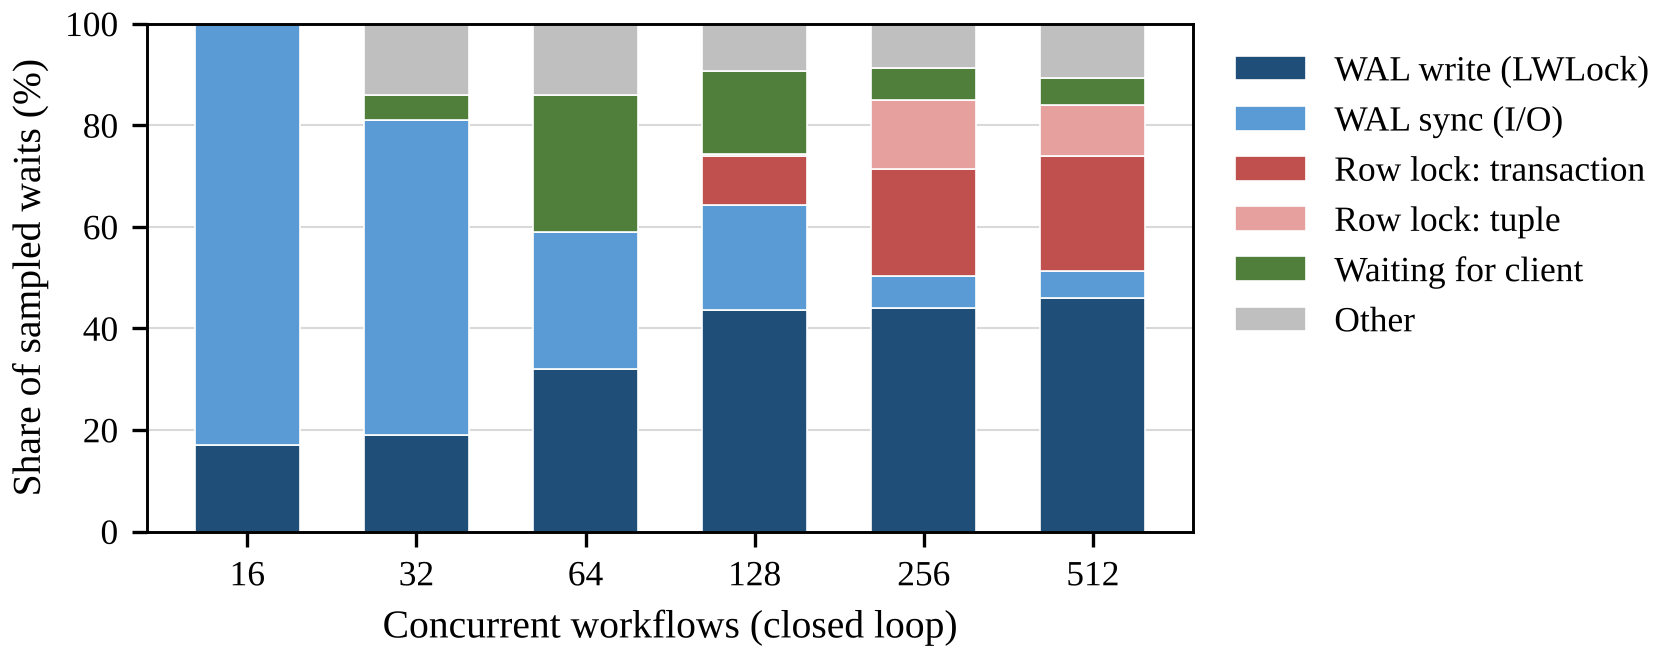
\includegraphics[width=0.9\linewidth]{figures/fig_7_3_db_waits.png}
  \caption[Database wait events]{Share of sampled database wait events by
    type (Stage~D).}
  \label{fig:waits}
\end{figure}

Dividing the commit rate by throughput gives about 100 database transactions
per completed workflow at the knee. A delivery workflow needs on the order of
fifteen writing transactions (start, four activity completions, the
decisions that follow them, a timer and the final decision); the remainder
are polls that found nothing or lost a race for a task. Reducing empty polls
is therefore the most direct way to raise capacity on a fixed database.

\section{Open-Loop Capacity and Overload}

Table~\ref{tab:open} and Fig.~\ref{fig:open} give the results when workflows
were offered at a fixed rate, from half to 1.1 times the closed-loop knee.
At 65.6 and 98.3 workflows/s every trial completed the offered load with a
median of 1.5\,s and p99 at or below 2.9\,s, lower than the floor at
$c=1$. From 108\,workflows/s upwards the behaviour became unstable: in most
trials completed throughput fell well below the offered rate, thousands of
starts were dropped and p99 rose to 40--56\,s, although an individual trial
at 108 and one at 144\,workflows/s kept up.

\begin{table}[htbp]
  \centering
  \caption{Open-loop results (three trials per rate)}
  \label{tab:open}
  \small
  \begin{tabular}{@{}rrrrr@{}}
    \toprule
    \textbf{Offered (wf/s)} & \textbf{Completed (wf/s)} & \textbf{Dropped} &
      \textbf{p99 (s)} & \textbf{Lease changes} \\
    \midrule
    65.6  & 64.6--64.9 & 0 & 2.2 & 0 \\
    98.3  & 96.9--97.2 & 0 & 2.2--2.9 & 0 \\
    108.2 & 67.6 / 76.3 / 106.8 & 3,340 / 2,507 / 0 & 44.5 / 45.2 / 2.7 &
      10 / 0 / 0 \\
    118.0 & 82--85 & 2,234--2,648 & 46--48 & 10 each \\
    131.1 & 67--99 & 2,700--5,889 & 43--51 & 10 / 28 / 10 \\
    144.2 & 75.0 / 102.8 / 128.8 & 5,849 / 3,010 / 0 & 55.9 / 44.6 / 39.0 &
      14 / 10 / 0 \\
    \bottomrule
  \end{tabular}
\end{table}

\begin{figure}[htbp]
  \centering
  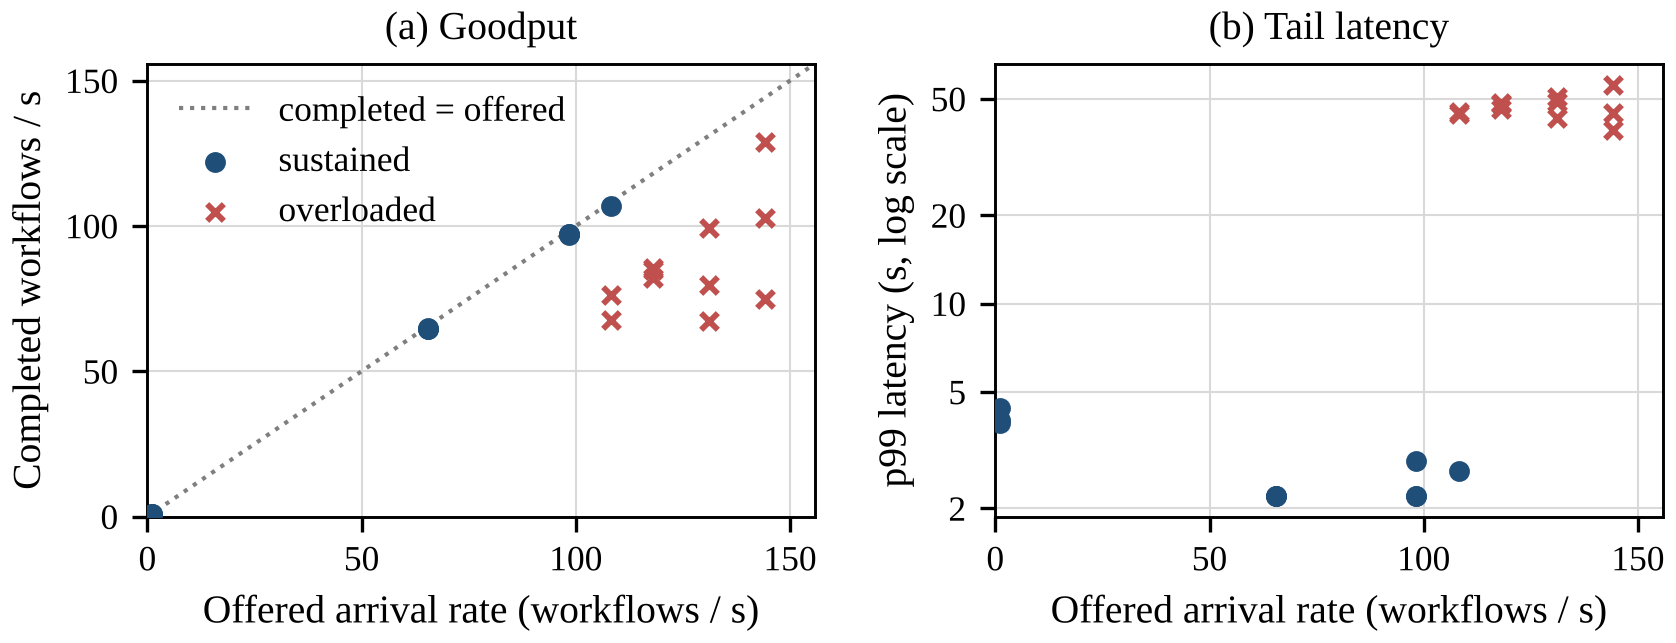
\includegraphics[width=0.9\linewidth]{figures/fig_7_4_open_loop.png}
  \caption[Open-loop offered against completed load]{Open-loop offered
    against completed load (Stage~E).}
  \label{fig:open}
\end{figure}

The sustainable open-loop rate is therefore about 100\,workflows/s, roughly
three quarters of the closed-loop knee. The difference is the one Schroeder
\emph{et al.}\ warn of~\cite{openclosed2006}: a closed loop throttles its own
arrivals as latency rises, so it never pushes the system as far past
saturation as an open loop does.

The most damaging form of overload was lease loss. In nine of the eleven
overloaded trials, one engine lost and re-acquired its five shard leases, and
starts sent to those shards in the meantime were refused with
\cd{NotOwner}. Closed-loop runs never lost a lease, even at 96\% database CPU.
Our hypothesis, which these runs do not prove, is that with the pools
60--73\% empty and the database above 85\% CPU, a renewal waited long enough
for a connection to miss the 10\,s lease. If so, lease renewal should be
given its own connection, separate from the pool used by workers. In every
overloaded trial, safety held: no invariant was violated, refused starts were
never accepted, and every accepted run completed. Overload cost availability
and latency, not correctness.

\section{Sensitivity to Workers, Shards and Replicas}

Fig.~\ref{fig:sens} and Table~\ref{tab:sens} show the capacity at $c=256$ as
each parameter was varied with the others at their defaults. Worker count
has an optimum. With 2+4 workers per shard the database still had headroom
(76\% CPU) and the workers were the bottleneck; with 8+16 the database spent
so much CPU on polling that capacity fell to 120\,workflows/s, although more
workers did reduce latency at moderate load. At a fixed total of 192 workers,
32 shards performed the same as 16, while 64 shards lost 13\%, again because
each shard adds polling and renewal work. Spreading the shards more evenly did
not help: the ring placed 5, 9 and 2 of the 16 shards on the three nodes, but
the limiting resource was the shared database, not the busiest engine.

\begin{figure}[htbp]
  \centering
  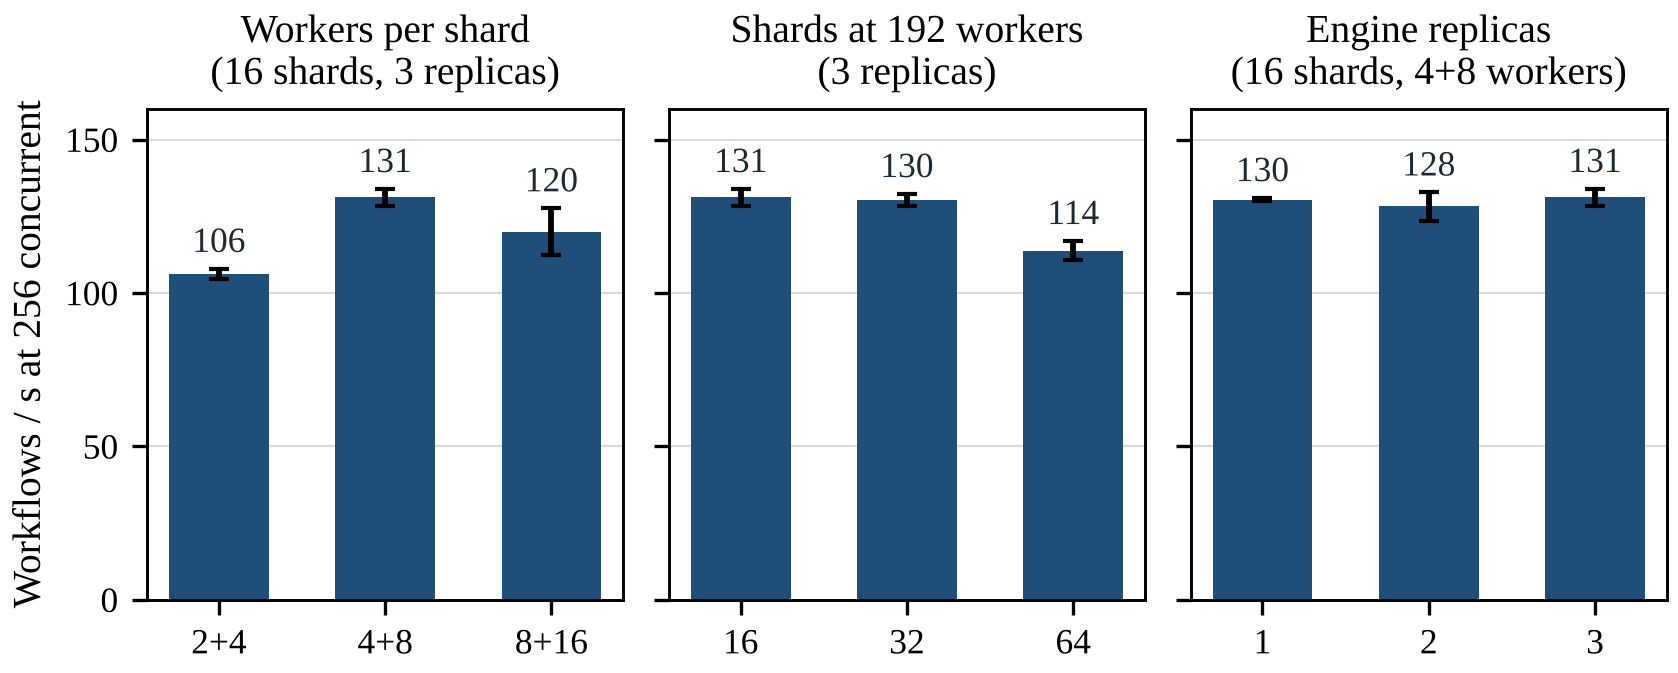
\includegraphics[width=\linewidth]{figures/fig_7_6_sensitivity.png}
  \caption[Sensitivity to workers, shards and replicas]{Capacity at $c=256$
    against workers, shards and replicas (Stages F, G and H).}
  \label{fig:sens}
\end{figure}

\begin{table}[htbp]
  \centering
  \caption{Capacity at $c=256$ under parameter changes (mean of three trials)}
  \label{tab:sens}
  \small
  \begin{tabular}{@{}llrr@{}}
    \toprule
    \textbf{Parameter} & \textbf{Value} & \textbf{Workflows/s} &
      \textbf{p99 (s)} \\
    \midrule
    Workers per shard & 2+4 & 106.2 & 3.4--4.1 \\
     & 4+8 (default) & 131.1 & 2.7--3.1 \\
     & 8+16 & 120.0 & 3.8--7.7 \\
    Shards (192 workers) & 32 & 130.3 & 2.8--3.4 \\
     & 64 & 113.8 & 3.9--4.5 \\
    Engine replicas & 1 & 130.4 & 2.7--3.0 \\
     & 2 & 128.2 & 2.6--3.7 \\
     & 3 (default) & 131.1 & 2.7--3.1 \\
    \bottomrule
  \end{tabular}
\end{table}

Adding replicas did not increase capacity: one, two and three replicas
reached 130.4, 128.2 and 131.1\,workflows/s. This is the expected result when
all replicas share one database that is already the bottleneck, and it should
not be read as a statement about horizontal scalability in general. Past the
knee, one replica actually did slightly better (140 against 124\,workflows/s
at $c=512$), because its single connection pool limited how many transactions
reached the database at once. Measuring horizontal scaling requires a
database that is not the limit, which was outside the budget of this
project.

\section{Recovery from Faults}

Table~\ref{tab:faults} and Fig.~\ref{fig:faults} summarise the 16 valid fault
trials. The cases fall into three groups.

\begin{table}[htbp]
  \centering
  \caption{Fault recovery under 65.6\,wf/s open-loop load}
  \label{tab:faults}
  \small
  \begin{tabular}{@{}p{1.15in}rrrrr@{}}
    \toprule
    \textbf{Fault} & \textbf{$t_\text{expire}$ (s)} & \textbf{$t_\text{claim}$ (s)}
      & \textbf{$t_\text{ring}$ (s)} & \textbf{Refused} & \textbf{p99 (s)} \\
    \midrule
    Graceful delete & 1.4--4.1 & 4.1--5.9 & 31.9--32.3 & 0--1 & 4.4--5.8 \\
    \cd{SIGKILL} & 4.7--5.3 & 4.7--5.3 & 34.6--36.8 & 0--1 & 2.2--3.3 \\
    Freeze 35\,s & 12.2--12.8 & 32.3--47.7 & 51.2--55.2 & 118--864 &
      31.9--46.2 \\
    Database sever & none & none & not broken & 0 & 2.2 \\
    Node drain & 4.2--8.3 & 23.1--23.9 & 38.5--49.7 & 176--736 & 4.8--6.7 \\
    Database reboot & 22.4 & 33.2 & 35.2 & 1,365 & 5.2 \\
    \bottomrule
  \end{tabular}
\end{table}

\begin{figure}[htbp]
  \centering
  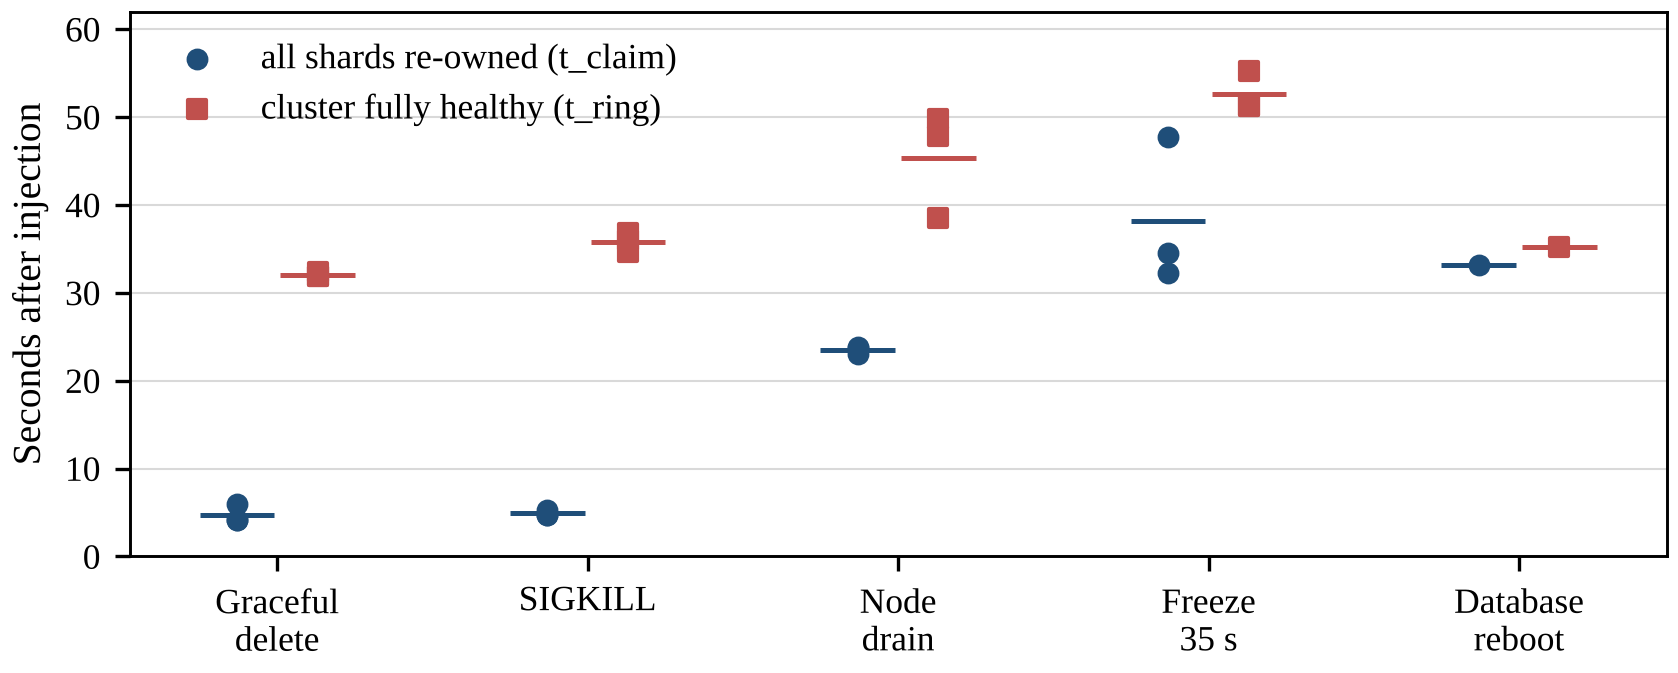
\includegraphics[width=0.9\linewidth]{figures/fig_7_7_fault_recovery.png}
  \caption[Recovery times by fault]{Time until all shards were re-owned and
    until the cluster was fully healthy, per fault.}
  \label{fig:faults}
\end{figure}

\paragraph{Fast handover.} After a graceful delete the victim released its
leases, and after \cd{SIGKILL} the restarted pod, which keeps its name in the
StatefulSet, re-acquired its own shards. In both cases all shards were held
again with a higher token within 4.1--5.9\,s, and load errors were at most one
start per trial. The remaining 30\,s before the cluster was fully healthy were
spent by Kubernetes on restarting and readiness, not by the engine.

\paragraph{Slow handover.} When an engine was frozen for 35\,s, its leases
expired after 12.2--12.8\,s, the 10\,s lease plus up to one renewal interval,
but the shards were not claimed by another node until 32--48\,s. This is the
orphan-adoption delay of Section~4.1.4: a survivor adopts a shard only after
its lease has been expired for more than twice the lease period. A drained
node's shards were re-owned in about 23\,s, and the database reboot took
33\,s for all 16 shards. In these cases, starts sent to an unowned shard were
refused (118 to 1,365 per trial), and for the freeze p99 rose to 32--46\,s.
The adoption delay was chosen to prevent needless handovers after short
pauses; these results show its cost, and a shorter delay, or one that
depends on whether the owner answers its health check, would reduce
unavailability after a real failure.

\paragraph{No handover.} Severing an engine's database connections did not
move any lease, because the engine reconnected within its renewal interval;
progress on its shards resumed within a few milliseconds.

The most important result concerns safety. When a frozen engine resumed, it
still believed it owned its shards, and it attempted to write to them. Those
writes were rejected by the fencing check 22, 4 and 5 times in the three
trials. Across all 16 valid trials no journal invariant was violated: there
were no duplicate sequence numbers, duplicate activity completions, sequence
gaps or runs with more than one terminal event, and every accepted run
completed after the load drained. Fencing therefore did what it was designed
to do on real infrastructure.

One engine defect was found. During one drain trial, the restarted engine's
start-up migration deadlocked with the other engines' live traffic; the
process exited and Kubernetes restarted it, after which the trial recovered
normally. Migrations should take an advisory lock and be skipped when the
schema is already current.

\section{Correctness Summary}

Over the closed- and open-loop stages, about 140,000 workflow runs were
checked by the journal invariants after their measurement points, together
with every run in the fault trials and the local duplicate audit. No
violation was found in any of them. This is evidence for these workloads and
faults; it is not a proof, and the runs did not include network partitions
between engines, which were not tested.

\section{Semantic Deduplication}

The duplicate check was evaluated in three steps: on the original flight
corpus, on corpora covering forty kinds of task, and inside the engine on
the cloud test bed.

\paragraph{One domain.} On the 213 flight pairs, exact matching never
suppressed a distinct request but caught only the 14 of 98 repeats that are
identical after normalisation. Pure semantic matching at the shipped
thresholds ($\tau_\text{low}=0.85$, $\tau_\text{high}=0.90$) judged 108 of
the 115 distinct pairs to be duplicates, including all 91 lexically close
ones, and no threshold between 0.70 and 0.99 separated the classes: the
encoder places ``BLR to DEL Friday morning'' as close to ``BLR to DEL
Saturday morning'' as to a genuine paraphrase. The hybrid comparator with
the flight field reader caught all 98 repeats with no false positive.

\paragraph{Many domains.} That flight result does not transfer. The flight
field reader was written by reading the flight corpus, and on the
ten-domain corpus of Section~6.3 it caught only 29 of 150 repeats while
suppressing 51 of 150 distinct actions, because outside flights it reads
nothing and falls back to pure similarity. A first value-shape reader
(generic-v1) caught 147 of 150 but still suppressed 40 of 150. Reading those
40 errors showed that the deciding detail was often a word (a payee, a city,
a service level, an action such as \emph{delete} against \emph{snapshot}), a
direction, or a value stated on one side only. Generic-v2
(Section~5.6) was designed from that analysis and then frozen, and it was
scored once on each of two corpora of ten further task kinds that had been
committed before it existed. Table~\ref{tab:semantic} gives the results.

\begin{table}[htbp]
  \centering
  \caption{Duplicate check on unseen task kinds (150 repeats and 150
    distinct actions per corpus)}
  \label{tab:semantic}
  \small
  \begin{tabular}{@{}llrr@{}}
    \toprule
    \textbf{Corpus} & \textbf{Comparator} & \textbf{Repeats caught} &
      \textbf{Distinct suppressed} \\
    \midrule
    Held-out 1 & Exact & 0 & 0 \\
     & Value shapes (generic-v1) & 128 (85\%) & 41 (27.3\%) \\
     & \textbf{Generic-v2} & 68 (45\%) & \textbf{5 (3.3\%)} \\
    Held-out 2 & Exact & 0 & 0 \\
     & Value shapes (generic-v1) & 115 (77\%) & 42 (28.0\%) \\
     & \textbf{Generic-v2.1} & 82 (55\%) & \textbf{3 (2.0\%)} \\
    \bottomrule
  \end{tabular}
\end{table}

On task kinds it had never seen, generic-v2 suppressed about one wrong
action in forty instead of one in four, at the price of catching only about
half of the reworded repeats. The repeats it misses are paraphrases that
swap ordinary words, such as \emph{pay} for \emph{transfer} or \emph{move}
for \emph{upgrade}; those are left to run, which is no worse than having no
semantic check, and the dedup key still reaches the downstream service. The
wrong suppressions that remain on the second held-out set were a seating
tier hidden after a count (``2 gold tickets'') and two reversed directions
phrased without ``to''.

\paragraph{Would a model help with the residue?} The pairs generic-v2 left
undecided were scored with the engine's embedding model on the cloud
operator. Calling such a pair a duplicate when its cosine reached 0.90 added
3 and 1 caught repeats on the two held-out sets, but raised the wrongly
suppressed actions from 1 to 10 and from 3 to 8 (generic-v2.1 throughout,
so held-out~1 is scored post hoc here); at 0.85 the cost was 19
and 10. The model does not separate a paraphrase from a one-word change of
identity any better than WordNet does, so it is not used to decide.

\paragraph{Inside the engine.} With generic-v2 configured, 12,173
\cd{DomainAgent} runs on the cloud test bed replayed every pair of the four
corpora through the engine's own path at 101 workflows/s. The rates matched
the offline evaluation (held-out 1: 44\% of repeats suppressed, 0.7\% of
distinct actions; held-out 2: 55\% and 1.9\%), and in no run did the
journalled verdict disagree with the number of times the action really
executed. Writing that workload exposed two defects in the semantic path,
both since fixed with regression tests: a suppressed call journalled the
reused result but never woke the workflow, so a run whose only pending step
was suppressed stopped for ever; and the intent stored for a completed call
was rendered differently from the live query it would later be compared
with.

\section{Threats to Validity}
\label{sec:validity}

Several factors limit how far these results can be generalised. All
measurements were taken in one availability zone, on one day per campaign,
on burstable ``flex'' instances whose performance can vary over time; trials
were repeated three times but not across days. Each measurement point lasted
two minutes after warm-up, which is long enough to observe saturation but not
long-term effects such as table bloat or autovacuum. The database was a
single 2-vCPU host, so every capacity figure is a property of that host, and
nothing here bears on database high availability. Capacity was measured
with one workflow type, the mixed workloads at moderate load only. Finally, the semantic corpus was synthetic, as discussed
above.
